\section{Introduction}
\begin{frame}{Introduction}
	What is small signal analysis?
	\begin{itemize}
		\item Analyzing circuits with input and output signals containing nonlinear elements.
		\item Input signal = DC bias + small AC signal.
		\item Output signal = DC bias + small AC signal.
		\item Goal: Relate input and output AC signals analytically. 
		\item Solution: Linearize nonlinear elements around DC operating point (small signal model).
		\item Analyze resulting linear circuit.
	\end{itemize}
\end{frame}
\note[itemize]{
		\item Linear electrical systems are well researched, allowing analytical solutions.
		\item Nonlinear elements complicate circuit theory.
		\item Linear approximations enable the use of standard circuit analysis tools.
		\item Approximation is valid only for small signals within a limited interval.
}

\begin{frame}{Introduction}
	\begin{figure}
		\centering
		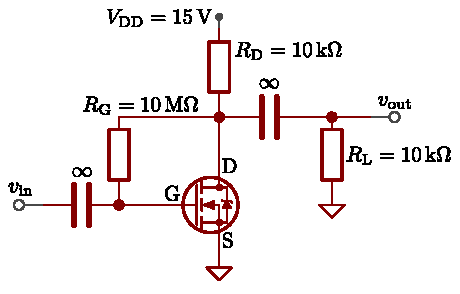
\includegraphics{../assets/example_circuit.pdf}
		\caption{Example circuit suitable for small signal analysis.}
		\label{fig:example_circuit}
	\end{figure}
\end{frame}